\section{Architecture Integration}

\subsection{Model Support}

\begin{table}[H]
\centering
\small
\begin{tabular}{llllll}
\toprule
\textbf{Architecture} & \textbf{Attention} & \textbf{Nested?} & \textbf{RoPE?} & \textbf{GQA?} & \textbf{Cross-attn?} \\
\midrule
DistilBERT & Flat & No & No & No & No \\
RoBERTa & Nested & Yes & No & No & No \\
GPT-2 & Causal & No & No & No & No \\
Qwen3.5 & GQA+RoPE & No & Yes & Yes & No \\
T5 & Enc-Dec & No & No & No & Yes \\
\bottomrule
\end{tabular}
\end{table}

\subsection{Weight Extraction}

\subsubsection{DistilBERT}
\begin{lstlisting}
q_w = src.q_lin.weight
k_w = src.k_lin.weight
v_w = src.v_lin.weight
o_w = src.out_lin.weight
\end{lstlisting}

\subsubsection{RoBERTa (Nested)}
\begin{lstlisting}
q_w = src.self.query.weight
k_w = src.self.key.weight
v_w = src.self.value.weight
o_w = src.output.dense.weight  # Only for reference
is_nested_encoder = True
\end{lstlisting}

\subsubsection{GPT-2 (Conv1D)}
\begin{lstlisting}
w = src.c_attn.weight.T  # (2304, 768)
q_w, k_w, v_w = w.chunk(3, dim=0)
o_w = src.c_proj.weight.T
\end{lstlisting}

\subsubsection{Qwen (GQA + RoPE)}
\begin{lstlisting}
q_w = src.q_proj.weight
k_w = src.k_proj.weight
v_w = src.v_proj.weight
o_w = src.o_proj.weight
num_kv_heads = config.num_key_value_heads
\end{lstlisting}

\subsection{Nested Encoder Handling}

For RoBERTa/BERT, \texttt{is\_nested\_encoder = True}:

\begin{lstlisting}
if self.is_nested_encoder:
    final_out = out  # Skip out_proj
else:
    final_out = self.out_proj(out)
\end{lstlisting}

The outer \texttt{BertSelfOutput.dense} applies its projection.

\subsection{Partial RoPE}

For Qwen3.5 with rotary\_dim < head\_dim:

\begin{lstlisting}
q_rot, q_pass = q[..., :rotary_dim], q[..., rotary_dim:]
q_rot = (q_rot * cos) + (rotate_half(q_rot) * sin)
q = torch.cat([q_rot, q_pass], dim=-1)
\end{lstlisting}

\subsection{Causality}

\begin{lstlisting}
causal_flag = bool(self.is_decoder and not is_cross_attention and L == kv_len)
\end{lstlisting}

\begin{itemize}
\item If decoder self-attention with L == kv\_len: apply causal.
\item Cross-attention: no causal mask.
\item Encoder self-attention: no causal mask.

\end{itemize}
\subsection{Cross-Attention}

For encoder-decoder models:

\begin{lstlisting}
kv_input = encoder_hidden_states
# No causal masking
\end{lstlisting}

\subsection{Registry}

\begin{lstlisting}
@ATTENTION_REGISTRY.register("flash3")
@ATTENTION_REGISTRY.register("flash_attention3")
class FlashAttention3(BaseAttention):
    ...
\end{lstlisting}

\subsection{Failure Modes}

\begin{table}[H]
\centering
\small
\begin{tabular}{lll}
\toprule
\textbf{Failure} & \textbf{Detection} & \textbf{Response} \\
\midrule
FA3 not installed & ImportError & SDPA fallback \\
FA3 kernel fails & try/except & SDPA fallback \\
FP8 unsupported & hasattr check & FP16 \\
Missing weights & Frobenius check & Warning + skip \\
Shape mismatch & Reshape attempt & Broadcast fallback \\
\bottomrule
\end{tabular}
\end{table}

\subsection{Dispatch Logic}

\begin{lstlisting}
if FLASH_ATTN_AVAILABLE and hidden_states.is_cuda:
    try:
        out = flash_attn_func(q, k, v, causal=causal_flag)
    except Exception:
        out = None
else:
    out = None

if out is None:
    out = F.scaled_dot_product_attention(q, k, v, ...)
\end{lstlisting}

\subsection{Numerical Precision}

\begin{lstlisting}

---
\end{lstlisting}

\begin{figure}[H]
\centering
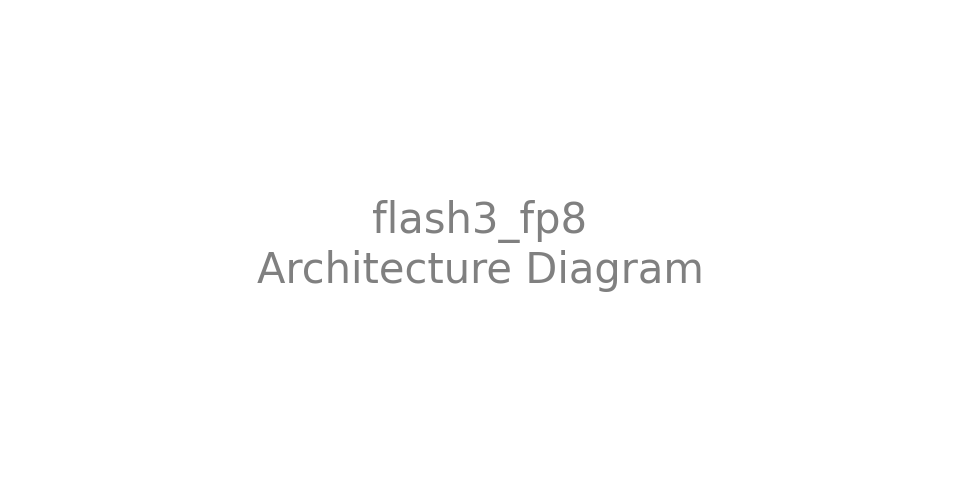
\includegraphics[width=\linewidth]{figures/architecture.png}
\caption{High-level architectural diagram of flash3.}
\label{fig:arch_flash3}
\end{figure}

